\documentclass[11pt,a4paper]{article}
\usepackage{TeX_definitions}
\geometry{left=2.4cm,right=2.4cm,top=2.4cm,bottom=2.4cm}
\graphicspath{{figures/}}
\hypersetup{colorlinks=true,linkcolor=blue,citecolor=blue,urlcolor=blue}

\title{Analysis 4-5: does a two-stage query-plus-belief task provide stronger behavioural constraints?}
\author{}
\date{\today}
\begin{document}
\maketitle

\section{Question}
Analysis 4-5 asks whether a richer behavioural paradigm can improve model discrimination. The tested candidate is a fixed-evidence task in which the participant first chooses which node to answer and then reports a belief for that node.

\section{Method}
Standard graphical-model background and notation are treated in the usual way; see \cite{Koller2009}.


We constructed partial-evidence versions of the reduced panel from Analysis 4-2. Each family chose a target by maximising model-specific certainty under its own posterior, then produced a belief report on that chosen node. We compared three designs: forced-target belief only, selection only, and the combined selection-plus-belief design.

\section{Results}
The mean pairwise family separation was 0.003211 for belief-only, 0.030576 for selection-only, and 0.054955 for the combined design. The joint design therefore adds a second diagnostic channel and raises average separation substantially above the forced-target baseline.

The recovery picture is more cautious. Under the present simple synthetic-noise model, the mean recovery diagonal was higher for belief-only than for the combined design. This means the two-stage task is promising as a targeted extension, but not yet a clear full replacement.

\begin{figure}[H]
\centering
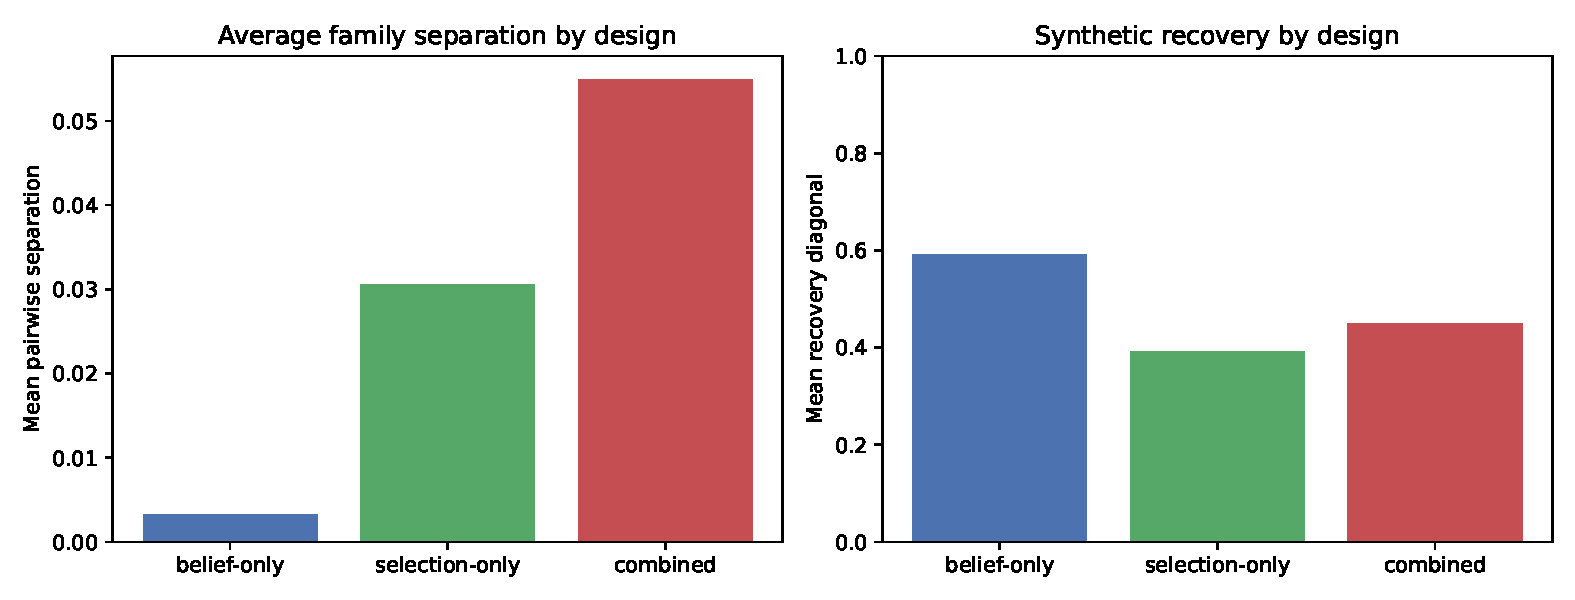
\includegraphics[width=\textwidth]{analysis-4-5_fig2_design_comparison.pdf}
\caption{Average separation and synthetic recovery under three candidate behavioural designs.}
\end{figure}

\section{Conclusions against the TODO}
\begin{enumerate}
    \item Selection behaviour is family-diagnostic on the partial-evidence panel.
    \item The combined design increases average pairwise family separation relative to belief-only.
    \item The fixed-evidence choose-node-then-report-belief format is the cleanest richer extension.
    \item The current evidence supports treating it as a targeted supplement to forced-target trials rather than an immediate replacement.
\end{enumerate}

\bibliographystyle{apalike}
\bibliography{../../manuscript/library}
\end{document}
